% Figure: Deterministic Boundary Checklist
% Source: originally in sections/deterministic_logic.tex (second figure)
% Depicts: AI proposed mapping → debit/credit check → liquidity boundary →
%          Approved OR Raise Audit Flag.
\begin{figure}[ht]
\centering
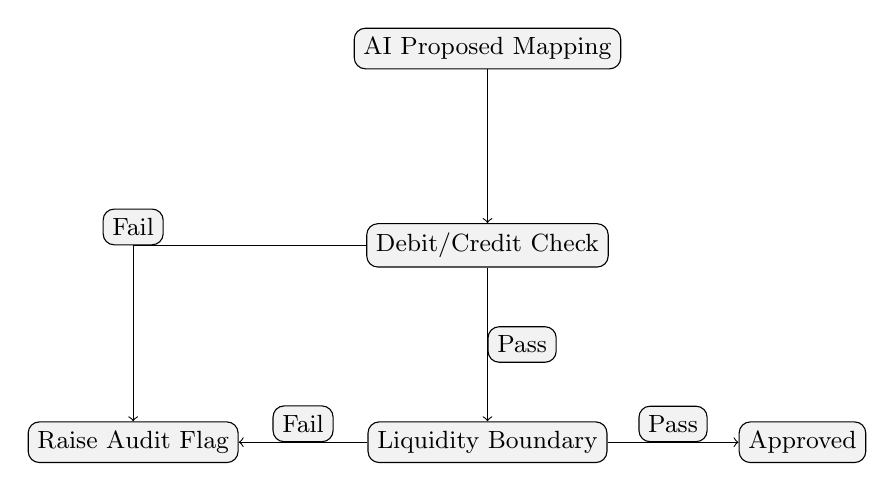
\begin{tikzpicture}[node distance=2.5cm, every node/.style={draw, fill=gray!10, rounded corners, font=\small}]
    \node (step1) {AI Proposed Mapping};
    \node (step2) [below of=step1] {Debit/Credit Check};
    \node (step3) [below of=step2] {Liquidity Boundary};
    \node (success) [right of=step3, node distance=4cm] {Approved};
    \node (fail) [left of=step3, node distance=4.5cm] {Raise Audit Flag};

    \draw[->] (step1) -- (step2);
    \draw[->] (step2) -- node[right] {Pass} (step3);
    \draw[->] (step3) -- node[above] {Pass} (success);
    \draw[->] (step2) -| node[above] {Fail} (fail);
    \draw[->] (step3) -- node[above] {Fail} (fail);
\end{tikzpicture}
\caption{The deterministic boundary checklist verifies AI-proposed mappings prior to ledger write-in.}
\label{fig:deterministic_checklist}
\end{figure}
